\documentclass[11pt]{article}
\usepackage[utf8]{inputenc}
\usepackage[T1]{fontenc}
\usepackage{lmodern}
\usepackage[margin=1in]{geometry}
\usepackage{amsmath,amssymb,amsthm}
\usepackage{graphicx}
\usepackage{booktabs}
\usepackage[hidelinks]{hyperref}
\usepackage{microtype}
\newtheorem{proposition}{Proposition}
\title{Single-Step Attacks Overstate the Adversarial Robustness of Angle-Encoded Quantum Classifiers}
\author{Michael Koppelmann}
\date{November 2026 $\cdot$ Draft $\cdot$ Created with Claude Code}
\begin{document}
\maketitle
\begin{abstract}
Several studies report that variational quantum classifiers resist adversarial examples better than classical networks, often on the basis of single-step or few-step gradient attacks. We revisit this claim for angle-encoded classifiers with data re-uploading, applying the gradient-masking checklist from the adversarial machine learning literature: iterative attacks with restarts, a line search along the single-step direction, a gradient-free attack, transfer attacks and an unbounded sanity check. Across 15 trained runs of each model (3 qubit counts: 5 seeds at $n=4$, 5 seeds at $n=6$, 5 seeds at $n=8$), FGSM leaves the quantum classifier at 44\% accuracy at $\varepsilon=0.3$, while 50-step PGD with restarts reduces it to 0\%; under the strong attack the quantum model is \emph{less} robust than a classical MLP at $\varepsilon=0.2$ (2\% vs 16\%), reversing the ranking FGSM suggests. Gradients are not obfuscated: the gradient-free attack beats white-box PGD in only 1 of 60 run--budget pairs, at $\varepsilon=0.05$, and unbounded attacks leave at most 6\% accuracy. Instead, the single-step attack fails because angle encoding makes the model a trigonometric polynomial of its input, whose curvature inside the threat ball grows with the encoding frequency and the perturbation budget, as a Bernstein-type bound predicts. Lowering the encoding frequency all but removes the effect (FGSM$-$PGD gap +0.02 at $s=0.25$ vs +0.52 at $s=1.5$), and a classical network given the same sinusoidal features shows the same failure in kind, at 20\%--49\% of the quantum model's magnitude. The apparent robustness comes from a weak attack meeting a periodic encoding, not from genuine robustness. We recommend iterative, multi-restart evaluation as the minimum standard for robustness claims about quantum classifiers.
\end{abstract}

\section{Introduction}\label{sec:intro}
Adversarial examples, inputs altered by small perturbations that change a model's prediction~\cite{goodfellow2015,madry2018}, are a central security concern for machine learning. As quantum machine learning matures, a growing literature asks whether quantum classifiers are more or less vulnerable than classical ones~\cite{liu2020,lu2020}. Several works report an advantage: quantum variational classifiers resisting attacks crafted on classical networks~\cite{west2022}, measured robustness on superconducting hardware attributed to noise-induced gradient attenuation~\cite{hwbench2025}, and defenses that deliberately hide gradients through randomized encodings~\cite{gong2022}. A recent systematization finds the opposite under white-box attacks~\cite{sok2025}.

Classical adversarial machine learning learned, at some cost, that apparent robustness is often an artifact of the evaluation. Defenses that \emph{mask} gradients, making them uninformative to the attacker without making the model robust, repeatedly passed gradient-based evaluations and then fell to adaptive attacks~\cite{athalye2018,uesato2018,tramer2020}. The resulting evaluation guidelines~\cite{carlini2019,croce2020} are rarely applied in full to quantum models. Of the works above, none reports the standard masking diagnostics for angle-encoded classifiers.

We apply them. Our subject is the most common architecture in the quantum adversarial literature: angle encoding with data re-uploading~\cite{perezsalinas2020} followed by strongly entangling layers~\cite{schuld2020}. Our contributions are:

\begin{itemize}
\item \textbf{A full gradient-masking evaluation} of angle-encoded variational quantum classifiers (VQCs) across 3 qubit counts and multiple seeds, comparing FGSM, FGSM with line search, PGD with restarts, the gradient-free SPSA attack, transfer attacks and unbounded attacks.
\item \textbf{Evidence that single-step attacks overstate VQC robustness}, to the point of reversing the robustness ranking against a classical network.
\item \textbf{A mechanism.} Angle encoding makes the classifier a trigonometric polynomial of its input. A Bernstein-type bound links the curvature inside the threat ball to the encoding frequency and perturbation budget, explaining when a single gradient-sign step overshoots.
\item \textbf{A classical control that isolates the cause.} An MLP on sinusoidal features with the same frequency content (SinMLP) reproduces the effect in kind, and an encoding-frequency sweep shows the encoding frequency controls it in both models.
\end{itemize}
\section{Background}\label{sec:bg}
\subsection{Attacks and gradient masking}
Given a classifier with logit $f(x)$ and label $y\in\{-1,+1\}$, we use the margin $m(x)=y\,f(x)$; the input is misclassified when $m<0$. An $\ell_\infty$ attack with budget $\varepsilon$ seeks $x'$ with $\|x'-x\|_\infty\leq\varepsilon$ and $m(x')<0$. FGSM~\cite{goodfellow2015} takes one step $x'=x-\varepsilon\,\mathrm{sign}(\nabla_x m)$. PGD~\cite{madry2018} iterates smaller steps with projection, ideally from several random starts. \emph{Gradient masking}~\cite{athalye2018} describes models whose gradients mislead first-order attackers. Its symptoms include single-step attacks performing far worse than iterative ones, gradient-free or transfer attacks beating white-box attacks, and unbounded attacks failing to reach zero accuracy.

\subsection{Angle encoding as a Fourier series}
In a re-uploading circuit, each feature enters through rotations $R_Y(s\pi x_i)$ repeated in $L$ layers. Because the generator has eigenvalues $\pm 1/2$, the model output is a trigonometric polynomial in each feature, with integer frequencies $k\in\{-L,\dots,L\}$ in units of $s\pi$~\cite{schuld2021}:

\begin{equation}
f(x)=\sum_{\omega\in\{-L,\dots,L\}^n} c_\omega\, e^{\,i s\pi\, \omega\cdot x}.
\end{equation}
The function is smooth but oscillatory, and its oscillation rate is set by the encoding frequency $s$ and the number of re-uploads $L$. A ReLU network, by contrast, is piecewise linear.

\section{Why single-step attacks fail on periodic models}\label{sec:theory}
Restrict $f$ to the FGSM ray: $g(t)=m(x+t\varepsilon d)$ with $d=-\mathrm{sign}(\nabla_x m)\in\{-1,0,1\}^n$ and $t\in[0,1]$. Each term of the series contributes a frequency $s\pi\varepsilon\,(\omega\cdot d)$ in $t$, and $|\omega\cdot d|\leq Ln$.

\begin{proposition}[Bernstein bound along the attack ray]
Let $\Omega=s\pi\varepsilon L n$. Then $\sup_t|g''(t)|\leq\Omega^2\sup_t|g(t)|$, so the error of the first-order model used by FGSM satisfies $|g(1)-g(0)-g'(0)|\leq\tfrac{1}{2}\Omega^2\sup_t|g(t)|$.
\end{proposition}
\emph{Proof sketch.} $g$ is a finite sum of exponentials with frequencies in $[-\Omega,\Omega]$, hence an entire function of exponential type $\Omega$ bounded on the real line. Bernstein's inequality~\cite{boas1954} gives $\sup|g'|\leq\Omega\sup|g|$; applying it twice gives the bound, and Taylor's theorem gives the error. $\square$

The bound is loose in $n$, but its scaling is the point. The linear approximation behind FGSM degrades quadratically in $s\varepsilon$. Once $\Omega\gtrsim 1$ the margin along the ray can turn around before $t=1$, so a full step overshoots, and the sign of the gradient at $x$ stops describing the loss a distance $\varepsilon$ away. Iterative attacks re-linearize at every step and are unaffected. The argument uses only the input spectrum, so it applies equally to any classical model with sinusoidal features of the same frequencies. This motivates the SinMLP control.

The bound predicts three observable signatures: (i) a gap between FGSM and PGD that grows with $\varepsilon$; (ii) points whose margin along the FGSM ray is non-monotone; and (iii) a gap that grows with the encoding frequency $s$, in quantum and classical models alike.

\section{Experimental setup}\label{sec:setup}
\textbf{Data.} Handwritten digits 3 vs 8~\cite{digits}, reduced by PCA to $n\in\{4,6,8\}$ features (one per qubit) and scaled to $[0,1]$. Each seed draws a new 60/40 train/test split and a new initialisation.

\textbf{Models.} Table \ref{tab:models} lists the three models; all use $s=1$ unless stated. The VQC is simulated exactly with PennyLane~\cite{pennylane} and trained with PyTorch~\cite{pytorch} (Adam, 20 epochs); the classical models train for 60 epochs.

\begin{table}[t]
\centering
\caption{Models. SinMLP has the same input frequencies as the VQC but nothing quantum.}
\label{tab:models}
\small
\begin{tabular}{ll}
\toprule
\textbf{Model} & \textbf{Architecture} \\
\midrule
VQC & $R_Y(s\pi x_i)$ re-uploaded before each of $L=3$ strongly entangling layers; $\langle Z_0\rangle$ $\rightarrow$ logit \\
SinMLP & features $\sin(k s\pi x_i),\cos(k s\pi x_i)$, $k=1..3$ $\rightarrow$ MLP(32, 32) \\
MLP & MLP(32, 32) with ReLU on the raw features \\
\bottomrule
\end{tabular}
\end{table}

\textbf{Attacks.} All are $\ell_\infty$ attacks on the margin, with inputs clipped to $[0,1]$: FGSM; FGSM-LS, the worst point along the FGSM ray over 20 step sizes in $(0,\varepsilon]$; PGD-20; PGD-50x5 (50 steps, step $2.5\varepsilon/50$, 5 random restarts); SPSA~\cite{uesato2018} (40 iterations, 32 random directions); a transfer attack using PGD-50x5 examples crafted on the MLP; and unbounded PGD ($\varepsilon=1$, 100 steps). \emph{Worst case} counts a point as robust only if it survives every attack.

\textbf{Diagnostics.} For each model and $\varepsilon$ we report the FGSM-PGD gap, the share of that gap recovered by line search, the share of test points whose margin along the FGSM ray reaches its minimum before $t=1$ (non-monotone), whether SPSA or transfer beat PGD, and the unbounded accuracy.

\section{Results}\label{sec:results}
\subsection{FGSM overstates robustness and can reverse the ranking}
\begin{figure}[t]
\centering
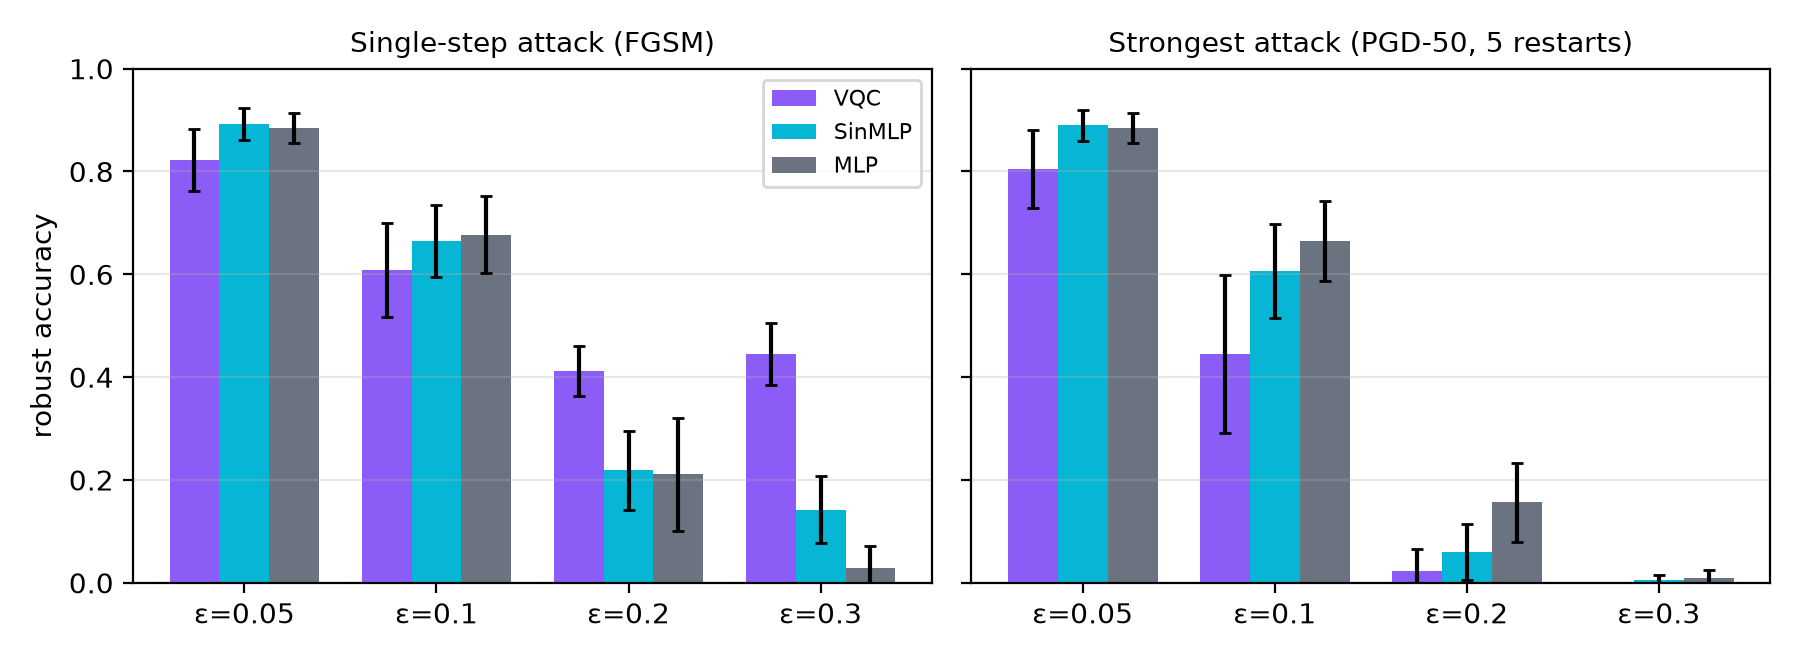
\includegraphics[width=0.95\linewidth]{figures/fig_ranking.png}
\caption{Robust accuracy (mean $\pm$ s.d. over all qubit counts and seeds) under the single-step attack (left) and the strongest white-box attack (right).}
\label{fig:ranking}
\end{figure}

Figure \ref{fig:ranking} and Table \ref{tab:main} summarise the main result. Under FGSM the VQC appears the most robust model at large budgets: 44\% accuracy at $\varepsilon=0.3$ versus 3\% for the MLP. Under PGD-50x5 it falls to 0\%. At $\varepsilon=0.2$ the ranking reverses: FGSM puts the VQC ahead of the MLP (41\% vs 21\%), PGD puts it behind (2\% vs 16\%). The worst case over all attacks is 0\% for the VQC, 0\% for the SinMLP and 1\% for the MLP at $\varepsilon=0.3$. Clean accuracy is similar across models (96\%, 97\%, 98\%).

\begin{table}[t]
\centering
\caption{Accuracy in \% (mean $\pm$ s.d. over seeds) under FGSM and PGD-50x5 at $\varepsilon=0.2$ and $\varepsilon=0.3$, and the worst case over all six attacks.}
\label{tab:main}
\small
\begin{tabular}{llrrrrrrr}
\toprule
\textbf{n} & \textbf{Model} & \textbf{Seeds} & \textbf{Clean} & \textbf{FGSM 0.2} & \textbf{PGD 0.2} & \textbf{FGSM 0.3} & \textbf{PGD 0.3} & \textbf{Worst 0.3} \\
\midrule
4 & VQC & 5 & 97 $\pm$ 1 & 44 $\pm$ 4 & 6 $\pm$ 5 & 42 $\pm$ 4 & 0 $\pm$ 0 & 0 $\pm$ 0 \\
4 & SinMLP & 5 & 97 $\pm$ 1 & 29 $\pm$ 5 & 11 $\pm$ 6 & 22 $\pm$ 5 & 1 $\pm$ 1 & 1 $\pm$ 1 \\
4 & MLP & 5 & 97 $\pm$ 1 & 33 $\pm$ 9 & 25 $\pm$ 4 & 8 $\pm$ 4 & 3 $\pm$ 2 & 2 $\pm$ 2 \\
6 & VQC & 5 & 98 $\pm$ 1 & 38 $\pm$ 2 & 0 $\pm$ 0 & 45 $\pm$ 9 & 0 $\pm$ 0 & 0 $\pm$ 0 \\
6 & SinMLP & 5 & 98 $\pm$ 1 & 22 $\pm$ 5 & 5 $\pm$ 3 & 11 $\pm$ 4 & 0 $\pm$ 1 & 0 $\pm$ 0 \\
6 & MLP & 5 & 99 $\pm$ 1 & 17 $\pm$ 5 & 12 $\pm$ 4 & 1 $\pm$ 1 & 0 $\pm$ 0 & 0 $\pm$ 0 \\
8 & VQC & 5 & 95 $\pm$ 2 & 42 $\pm$ 6 & 0 $\pm$ 0 & 47 $\pm$ 2 & 0 $\pm$ 0 & 0 $\pm$ 0 \\
8 & SinMLP & 5 & 98 $\pm$ 1 & 14 $\pm$ 5 & 2 $\pm$ 1 & 10 $\pm$ 3 & 0 $\pm$ 0 & 0 $\pm$ 0 \\
8 & MLP & 5 & 98 $\pm$ 0 & 13 $\pm$ 5 & 10 $\pm$ 2 & 0 $\pm$ 0 & 0 $\pm$ 0 & 0 $\pm$ 0 \\
\bottomrule
\end{tabular}
\end{table}

\subsection{The gradient-masking checklist}
\begin{table}[t]
\centering
\caption{Gradient-masking diagnostics at $\varepsilon=0.3$, pooled over qubit counts and seeds. \emph{SPSA < PGD} is the share of runs where the gradient-free attack beat PGD-50x5; \emph{Unbounded} is the highest accuracy left by $\varepsilon=1$ PGD.}
\label{tab:checklist}
\small
\begin{tabular}{lrrrrrr}
\toprule
\textbf{Model} & \textbf{FGSM$-$PGD gap} & \textbf{Gap closed by LS} & \textbf{Non-monotone} & \textbf{SPSA < PGD} & \textbf{Transfer acc.} & \textbf{Unbounded} \\
\midrule
VQC & +0.44 & 43\% & 71\% & 0\% & 0.24 & 0.06 \\
SinMLP & +0.14 & 20\% & 44\% & 0\% & 0.04 & 0.13 \\
MLP & +0.02 & 0\% & 0\% & 0\% & 0.01 & 0.00 \\
\bottomrule
\end{tabular}
\end{table}

Table \ref{tab:checklist} separates two explanations. The large FGSM-PGD gap for the VQC (+0.44) is the classic masking symptom. Yet the other symptoms are absent. At $\varepsilon=0.3$ the gradient-free SPSA attack beats PGD in 0\% of VQC runs, and across all budgets the gradient-free attack beats white-box PGD in only 1 of 60 run--budget pairs, at $\varepsilon=0.05$. Transfer from the MLP is weaker than white-box PGD (accuracy 0.24), and unbounded attacks leave at most 0.06. The VQC's gradients are informative; iterative attacks using them succeed. What fails is the single linearization. On 71\% of test points the margin along the FGSM ray turns around before the full step. A line search along the same direction recovers only 43\% of the gap, so the gradient sign at $x$ is itself a poor guide a distance $\varepsilon$ away, as the curvature bound predicts.

The SinMLP, which shares the VQC's per-feature input frequencies but nothing quantum, shows the same symptoms in kind but smaller (pooled gap +0.14, 44\% non-monotone). Its gap is 49\% of the VQC's at $n=4$, 25\% of the VQC's at $n=6$, 20\% of the VQC's at $n=8$. The VQC's gap holds steady as $n$ grows (+0.42, +0.45, +0.47), while the SinMLP's shrinks. A plausible reason, which we leave to future work, is that the entangling layers give the VQC every combined frequency $\omega\cdot x$ across features directly, whereas the SinMLP sees per-feature frequencies and must build combinations in its hidden layers. The ReLU MLP shows a gap of only +0.02 and 0\% non-monotone points. The transfer results also qualify earlier observations that classical adversarial examples transfer poorly to quantum classifiers~\cite{west2022}: here too transfer is weaker than white-box PGD, but white-box PGD defeats the VQC completely, so poor transfer is not evidence of robustness.

\subsection{Mechanism: curvature from the encoding frequency}
\begin{figure}[t]
\centering
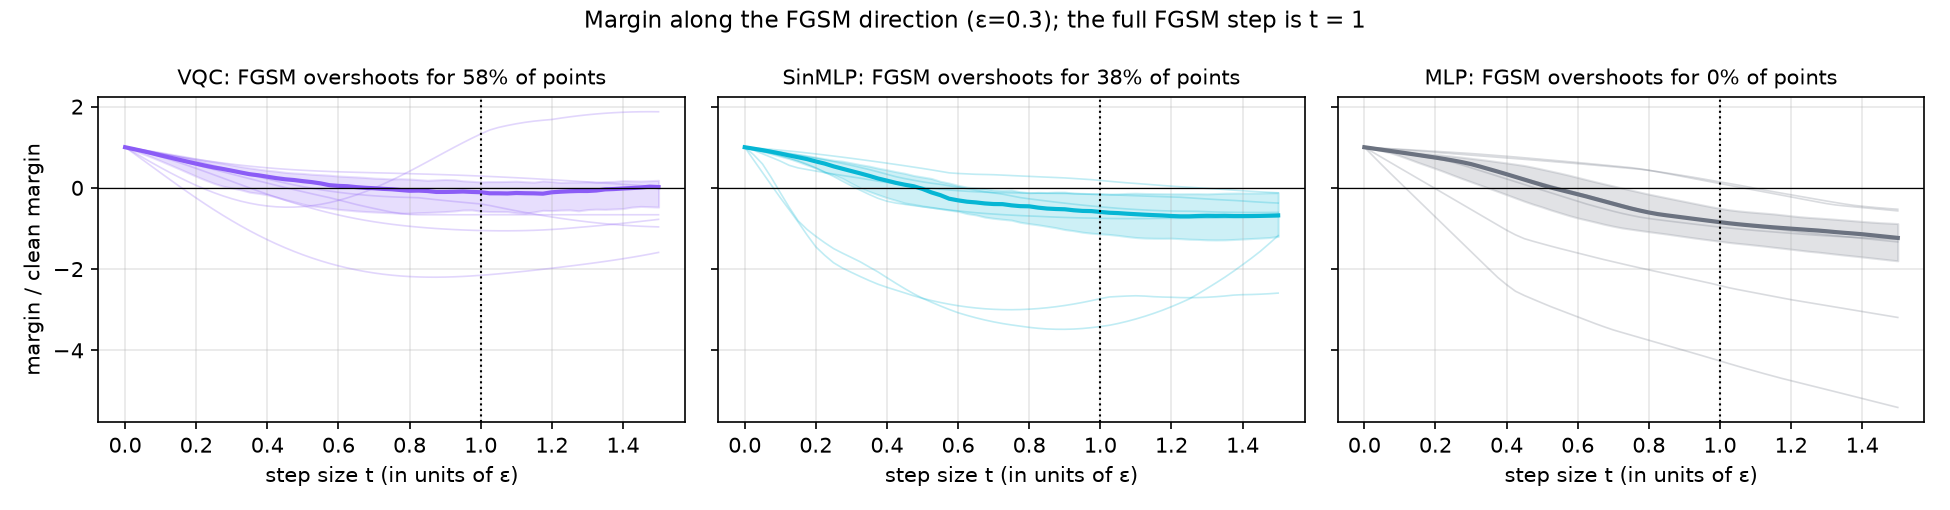
\includegraphics[width=1.00\linewidth]{figures/ray_profiles.png}
\caption{Margin along the FGSM direction, normalised by the clean margin, for correctly classified test points ($n=4$, $\varepsilon=0.3$). Thin lines: individual points; band: interquartile range; dotted line: the full FGSM step. Periodic models overshoot; the ReLU MLP does not.}
\label{fig:rays}
\end{figure}

Figure \ref{fig:rays} shows the overshoot directly. For the VQC the median margin along the FGSM ray flattens near zero well before the full step, and many individual points reach their minimum inside the threat ball and then turn back towards correct classification: FGSM overshoots on 58\% of points. The SinMLP overshoots on 38\% of points. The ReLU MLP's margin keeps falling along the whole ray, overshooting on 0\%.

\begin{figure}[t]
\centering
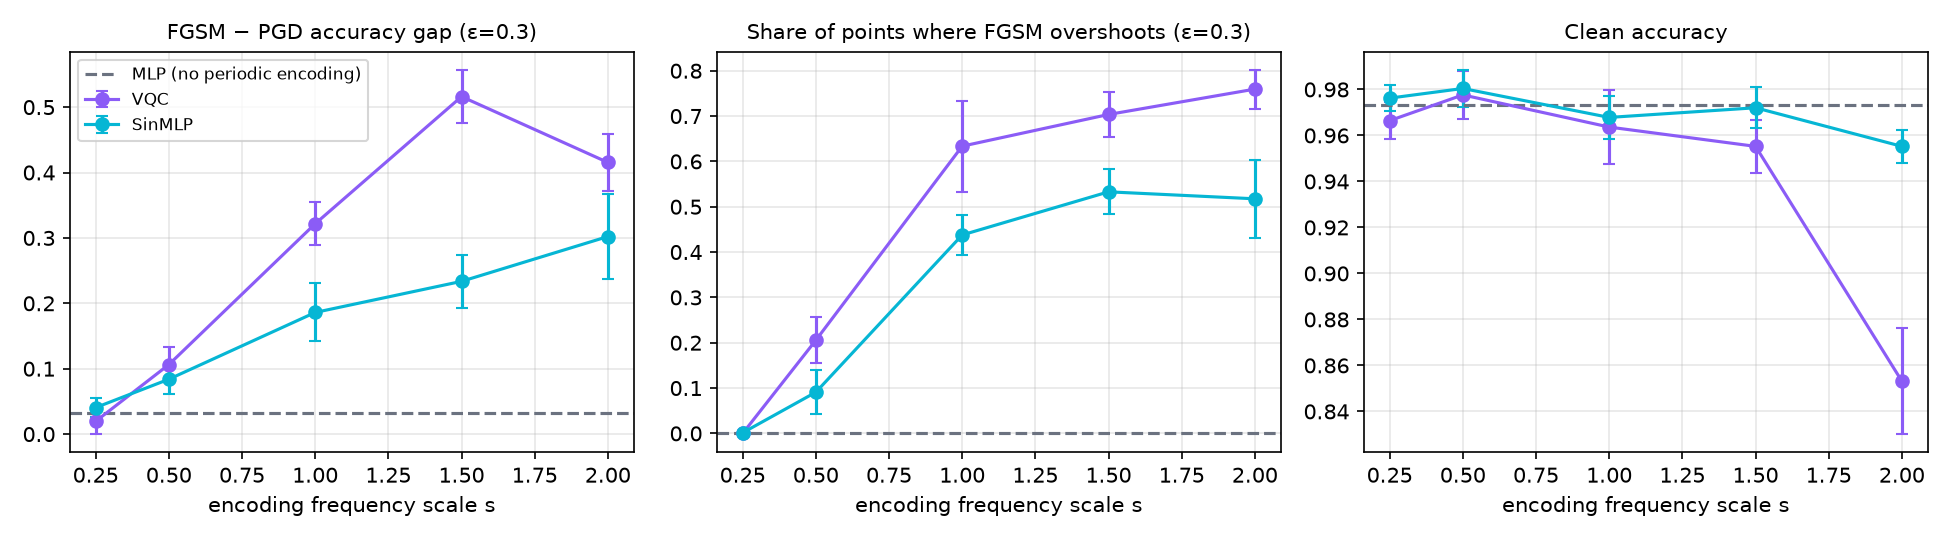
\includegraphics[width=1.00\linewidth]{figures/mechanism_sweep.png}
\caption{Encoding-frequency sweep ($n=4$, 5 seeds, $\varepsilon=0.3$). Left: FGSM$-$PGD gap; centre: share of points where FGSM overshoots; right: clean accuracy. Dashed: ReLU MLP.}
\label{fig:sweep}
\end{figure}

\begin{table}[t]
\centering
\caption{Encoding-frequency sweep at $\varepsilon=0.3$ (mean $\pm$ s.d. over 5 seeds).}
\label{tab:sweep}
\small
\begin{tabular}{rrrrrr}
\toprule
\textbf{s} & \textbf{VQC clean} & \textbf{VQC gap} & \textbf{VQC non-mono.} & \textbf{SinMLP gap} & \textbf{SinMLP non-mono.} \\
\midrule
0.25 & 0.97 $\pm$ 0.01 & 0.02 $\pm$ 0.02 & 0\% & 0.04 $\pm$ 0.01 & 0\% \\
0.5 & 0.98 $\pm$ 0.01 & 0.11 $\pm$ 0.03 & 21\% & 0.08 $\pm$ 0.02 & 9\% \\
1 & 0.96 $\pm$ 0.02 & 0.32 $\pm$ 0.03 & 63\% & 0.19 $\pm$ 0.04 & 44\% \\
1.5 & 0.96 $\pm$ 0.01 & 0.52 $\pm$ 0.04 & 70\% & 0.23 $\pm$ 0.04 & 53\% \\
2 & 0.85 $\pm$ 0.02 & 0.42 $\pm$ 0.04 & 76\% & 0.30 $\pm$ 0.06 & 52\% \\
\bottomrule
\end{tabular}
\end{table}

The sweep (Figure \ref{fig:sweep}, Table \ref{tab:sweep}) tests the causal prediction. Raising the encoding frequency from $s=0.25$ to $s=1.5$ raises the VQC's FGSM-PGD gap from +0.02 to +0.52; at $s=2$ it eases to +0.42 as clean accuracy falls to 85\% (from 96\% at $s=1$), which caps how large the gap can be. The SinMLP's gap rises from +0.04 to +0.30, while the ReLU MLP stays at +0.03. The share of overshooting points rises monotonically with $s$ for the VQC. Apparent FGSM robustness can therefore be dialled up or down through a classical hyperparameter of the encoding, with no change to the quantum part of the model.

\section{Discussion}\label{sec:discussion}
\textbf{What the results do and do not show.} They do not show that quantum classifiers are inherently less robust. Clean accuracy is matched, and the strongest attacks defeat all three models at large budgets. They show that FGSM is not a valid robustness measure for angle-encoded models: its failure is predictable from the encoding spectrum, vanishes at low encoding frequency, and appears in smaller form in classical models with the same per-feature spectrum. Robustness claims based on single-step attacks, or on attacks that are only weak against periodic models, should be re-examined.

\textbf{Relation to gradient masking.} In the taxonomy of~\cite{athalye2018} the effect is neither shattered nor stochastic gradients, and not vanishing gradients in the barren-plateau sense~\cite{mcclean2018}. It is high curvature: the gradient is correct but only locally useful. This is the benign form of masking: standard iterative attacks remove it, and gradient-free attacks confirm that nothing else is hidden. Mechanisms that do hide gradients, such as hardware noise~\cite{hwbench2025} or randomized encodings~\cite{gong2022}, need the full adaptive-attack treatment~\cite{tramer2020}.

\textbf{Recommendations.} Robustness evaluations of quantum classifiers should report (i) iterative attacks with random restarts as the primary metric, (ii) the FGSM-PGD gap and an unbounded-attack sanity check, (iii) at least one gradient-free attack, and (iv) a classical baseline matched on input encoding, so that effects of the encoding are not credited to quantumness.

\section{Limitations}\label{sec:limits}
\begin{itemize}
\item Simulations are exact: no shot noise or hardware noise, which may add genuinely stochastic masking.
\item Scale is small: 4--8 qubits, one dataset (digits 3 vs 8, PCA-reduced) and one circuit family. Amplitude-encoded and larger models are not covered.
\item SPSA's budget bounds the strength of the gradient-free check; a stronger score-based attack (e.g. Square Attack, AutoAttack~\cite{croce2020}) would tighten it.
\item The Bernstein bound is worst-case and loose in $n$; we use it for its scaling in $s\varepsilon$, which the sweep tests, not for its constant.
\end{itemize}
\section{Conclusion}\label{sec:conclusion}
Angle-encoded quantum classifiers look robust to single-step attacks because their periodic encoding makes the loss curve inside the threat ball, not because they are robust. Strong iterative attacks remove the effect, the encoding frequency controls it, and a classical model with the same encoding reproduces it in smaller form. Evaluations of quantum adversarial robustness should adopt the same standards as classical ones.

\section*{Reproducibility}
All code, raw results and this manuscript's build script are available at https://github.com/XxPacificxX/QuAIsar. The experiments run on a laptop CPU: masking\_study.py produces Tables \ref{tab:main}--\ref{tab:checklist} and mechanism.py produces the mechanism figures. Every number in this paper is generated from the saved results files.

\section*{Use of AI tools}
The experiment code, analysis and an initial draft of this manuscript were created with Claude Code (Anthropic). The author directed the research, reviewed the code, results and text, and takes full responsibility for the content.

\begin{thebibliography}{99}
\bibitem{goodfellow2015} I. J. Goodfellow, J. Shlens, and C. Szegedy. Explaining and harnessing adversarial examples. ICLR, 2015.
\bibitem{madry2018} A. Madry, A. Makelov, L. Schmidt, D. Tsipras, and A. Vladu. Towards deep learning models resistant to adversarial attacks. ICLR, 2018.
\bibitem{liu2020} N. Liu and P. Wittek. Vulnerability of quantum classification to adversarial perturbations. Physical Review A, 101:062331, 2020.
\bibitem{lu2020} S. Lu, L.-M. Duan, and D.-L. Deng. Quantum adversarial machine learning. Physical Review Research, 2:033212, 2020.
\bibitem{west2022} M. T. West, S. M. Erfani, C. Leckie, M. Sevior, L. C. L. Hollenberg, and M. Usman. Benchmarking adversarially robust quantum machine learning at scale. arXiv:2211.12681, 2022.
\bibitem{hwbench2025} Experimental robustness benchmarking of quantum neural networks on a superconducting quantum processor. arXiv:2505.16714, 2025.
\bibitem{gong2022} W. Gong, D. Yuan, W. Li, and D.-L. Deng. Enhancing quantum adversarial robustness by randomized encodings. arXiv:2212.02531, 2022.
\bibitem{sok2025} SoK: Critical evaluation of quantum machine learning for adversarial robustness. arXiv:2511.14989, 2025.
\bibitem{athalye2018} A. Athalye, N. Carlini, and D. Wagner. Obfuscated gradients give a false sense of security: Circumventing defenses to adversarial examples. ICML, 2018.
\bibitem{uesato2018} J. Uesato, B. O'Donoghue, P. Kohli, and A. van den Oord. Adversarial risk and the dangers of evaluating against weak attacks. ICML, 2018.
\bibitem{tramer2020} F. Tramèr, N. Carlini, W. Brendel, and A. Madry. On adaptive attacks to adversarial example defenses. NeurIPS, 2020.
\bibitem{carlini2019} N. Carlini, A. Athalye, N. Papernot, W. Brendel, J. Rauber, D. Tsipras, I. Goodfellow, A. Madry, and A. Kurakin. On evaluating adversarial robustness. arXiv:1902.06705, 2019.
\bibitem{croce2020} F. Croce and M. Hein. Reliable evaluation of adversarial robustness with an ensemble of diverse parameter-free attacks. ICML, 2020.
\bibitem{perezsalinas2020} A. Pérez-Salinas, A. Cervera-Lierta, E. Gil-Fuster, and J. I. Latorre. Data re-uploading for a universal quantum classifier. Quantum, 4:226, 2020.
\bibitem{schuld2020} M. Schuld, A. Bocharov, K. M. Svore, and N. Wiebe. Circuit-centric quantum classifiers. Physical Review A, 101:032308, 2020.
\bibitem{schuld2021} M. Schuld, R. Sweke, and J. J. Meyer. Effect of data encoding on the expressive power of variational quantum-machine-learning models. Physical Review A, 103:032430, 2021.
\bibitem{boas1954} R. P. Boas, Jr. Entire Functions. Academic Press, 1954.
\bibitem{digits} E. Alpaydin and C. Kaynak. Optical recognition of handwritten digits. UCI Machine Learning Repository, 1998.
\bibitem{pennylane} V. Bergholm et al. PennyLane: Automatic differentiation of hybrid quantum-classical computations. arXiv:1811.04968, 2018.
\bibitem{pytorch} A. Paszke et al. PyTorch: An imperative style, high-performance deep learning library. NeurIPS, 2019.
\bibitem{mcclean2018} J. R. McClean, S. Boixo, V. N. Smelyanskiy, R. Babbush, and H. Neven. Barren plateaus in quantum neural network training landscapes. Nature Communications, 9:4812, 2018.
\end{thebibliography}
\end{document}